\subsection{OSG View}
\label{sec:osgview}

The OSG View allows a graphical representation of target reports from the Database Objects. After creation, it displays a world map in the map widget on the left, supported by a configuration panel on the right hand side.

\begin{figure}[H]
    \hspace*{-2cm}
    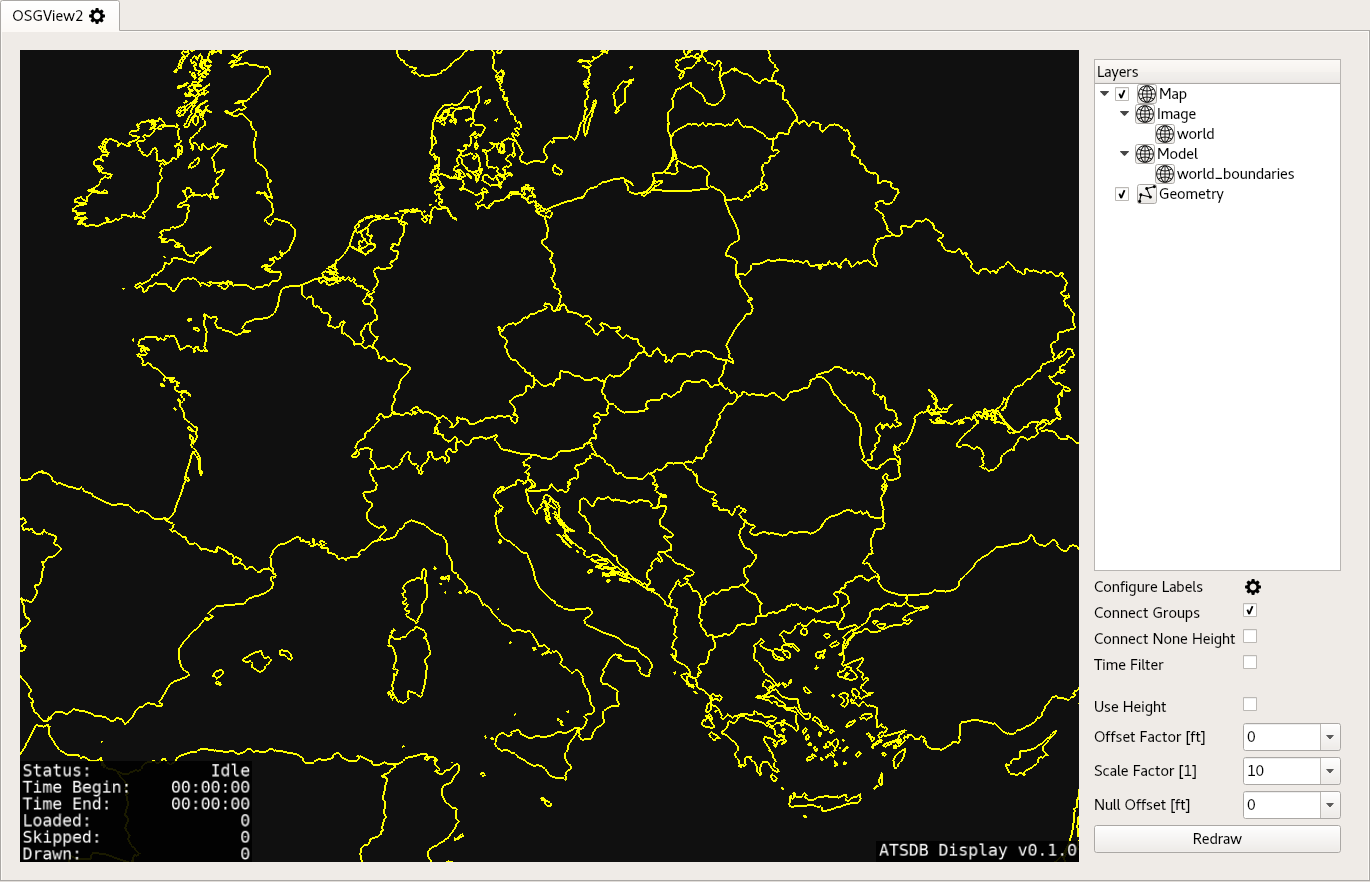
\includegraphics[width=18cm,frame]{../screenshots/osgview_overview.png}
  \caption{OSG View overview}
  \label{fig:osgview_overview}
\end{figure}

The map window will automatically traverse to the medium location of the data in the current database.

After loading, the target reports will be shown.

\begin{figure}[H]
    \hspace*{-2cm}
    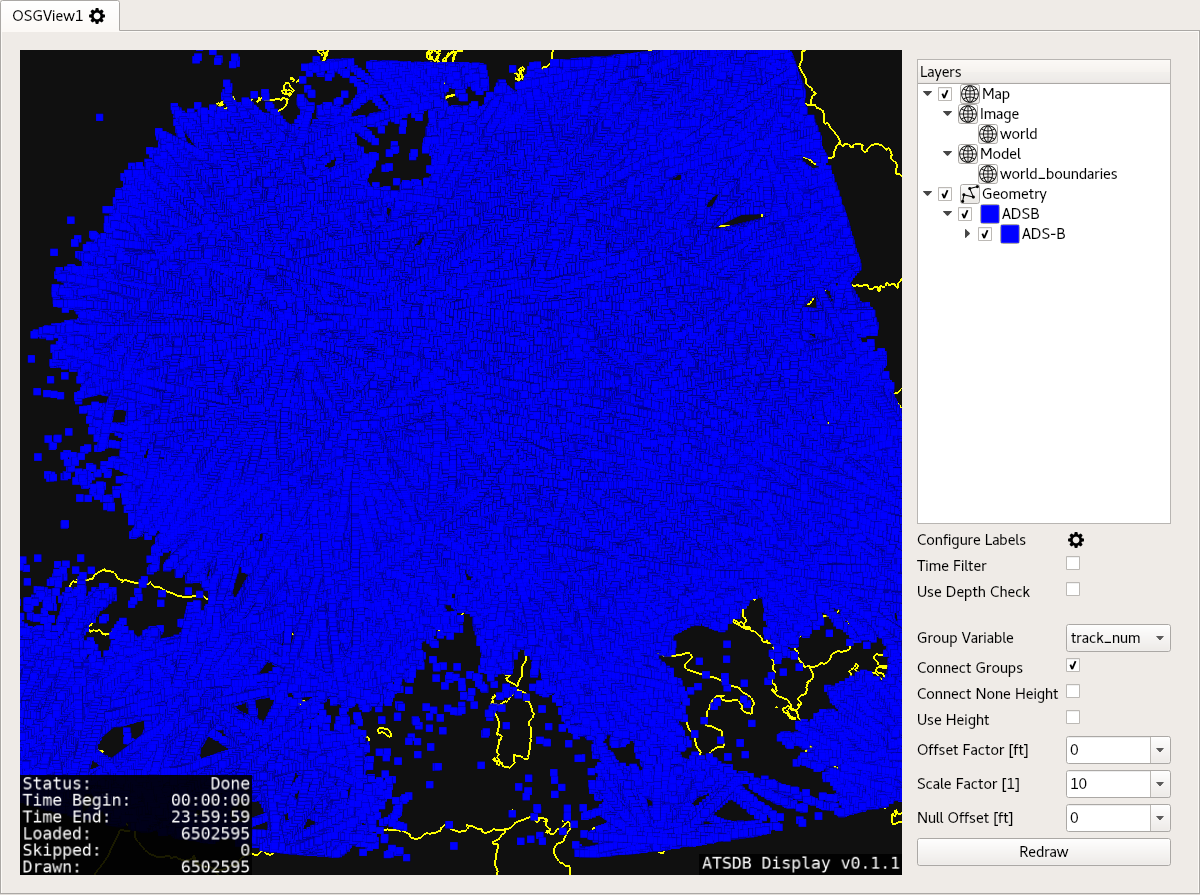
\includegraphics[width=18cm,frame]{../screenshots/osgview_overview_loaded.png}
  \caption{OSG View overview after loading}
\end{figure}


\subsubsection{Map Widget}
\label{sec:osgview_map}

In the map widget, several mouse and key operations are supported. The following terms are used:

\begin{itemize}
 \item LMB: Left mouse button
 \item MMB: Middle mouse button
 \item RMB: Right mouse button
 \item CTRL: CTRL key
\end{itemize}

\begin{table}[H]
  \center
  \begin{tabular}{ | l | l | l |}
    \hline
    \textbf{Mouse Action} & \textbf{Key Action} &  \textbf{Description} \\ \hline
    Single click & - & - \\ \hline
    LMB click \& drag & - & Traverse map \\ \hline
    - & Arrows & Traverse map \\ \hline
    MMB click \& drag & - & Rotate map \\ \hline
    RMB click \& drag & - & Zoom map \\ \hline
    MMB scroll \& drag & - & Zoom map \\ \hline
    LMB double click & - & Zoom to clicked location \\ \hline
    RMB double click \& drag & - & Zoom away from clicked location \\ \hline
    - & Space bar & Return to home position \\ \hline
  \end{tabular}
  \caption{Map widget view operations}
\end{table}

Further operations are defined in section Map Widget Data Operations. \\

In the lower-left corner, the data status information is given:

\begin{itemize}
 \item Status
\begin{itemize}
 \item Idle: Nothing to do
 \item Loading: Loading in progress
 \item Done: Loading/redraw done
 \item Redrawing: Redraw in progress
\end{itemize}
 \item Time Begin: First timestamp in the data, in HH:MM:SS
 \item Time End: last timestamp in the data, in HH:MM:SS
 \item Loaded: Number of loaded target reports (from the database)
 \item Skipped: Number of not-drawn target reports
 \item Loaded: Number of drawn target reports
\end{itemize}

In the lower-right corner, the ATSDB version is shown.

\subsubsection{Configuration Widget}
\label{sec:osgview_config}

In the configuration widget, several elements exist:

\begin{itemize}
 \item Layer widget: displays all currently existing layers
 \item Configuration area
\begin{itemize}
 \item Configure labels: Allows configuration of the labels
 \item Time Filter: Activates the Time Window Filter
 \item Use Depth Check: Activates line-of-sight depth check. Only recommended if height is used
 \item Group Variable: Meta DBOVariable used to create groups. Currently, only track number and Mode S address are supported
 \item Connect groups: Whether grouped target reports should be connected using lines
 \item Connect None Height: If groups are connected, whether target reports with not height information should be connected
 \item Use Height: Whether height information should be used to create a 3D presentation
 \item Offset Factor: If height information is used, this factor is added to the height
 \item Scale Factor: If height information is used, this factor is used to multiply the height
 \item Null Offset: If height information is used, this factor is used for target reports without height information
 \item Redraw button: Triggers a re-draw of the geometry, e.g. after a one of the above options was used
\end{itemize}
\end{itemize}

\subsubsection{Layer Widget}

In the layer widget, a tree view is given to configure the display of the existing elements. The following main tree elements are:
\begin{itemize}
 \item Map: Shows current map layers
 \item Geometry: Shows current DBO elements
\end{itemize}

\subsubsection{Changing the Background Map}

Please note that, while the default background map is supplied ATSDB, the other background map types are downloaded from public Internet sources and therefore require an Internet connection. They are then cached locally to facilitate faster access. \\

To change the background map, click the globe symbol {
\includegraphics[scale=0.05]{../../data/icons/globe.png} in Map Layer to access the map selection. The following maps are commonly available:

\begin{itemize}
 \item arcgis.earth
 \item minimal.earth
 \item openstreetmap.earth
 \item readymap.earth
 \item readymap-detailed.earth
\end{itemize}

The map loading and display in based on the osgEarth library (\url{http://osgearth.org/}), as are to map file definitions. The map which can be set using this dialog is simply a file list from the folder '~/.atsdb/data/maps'. So, changes can be made to the supplied ones or custom user maps can be added to this folder. \\
Please refer to \url{http://docs.osgearth.org/en/latest/references/earthfile.html} for a definition of an earth file.

\newpage
\paragraph{ArcGIS Map}

As supplied in the osgEarth example files, this map data is obtained from ArcGIS Online (\url{https://doc.arcgis.com/en/arcgis-online/reference/what-is-agol.htm}). It shows satellite imagery, supplied with elevation data from ReadyMap. 

\begin{figure}[H]
    \hspace*{-2cm}
    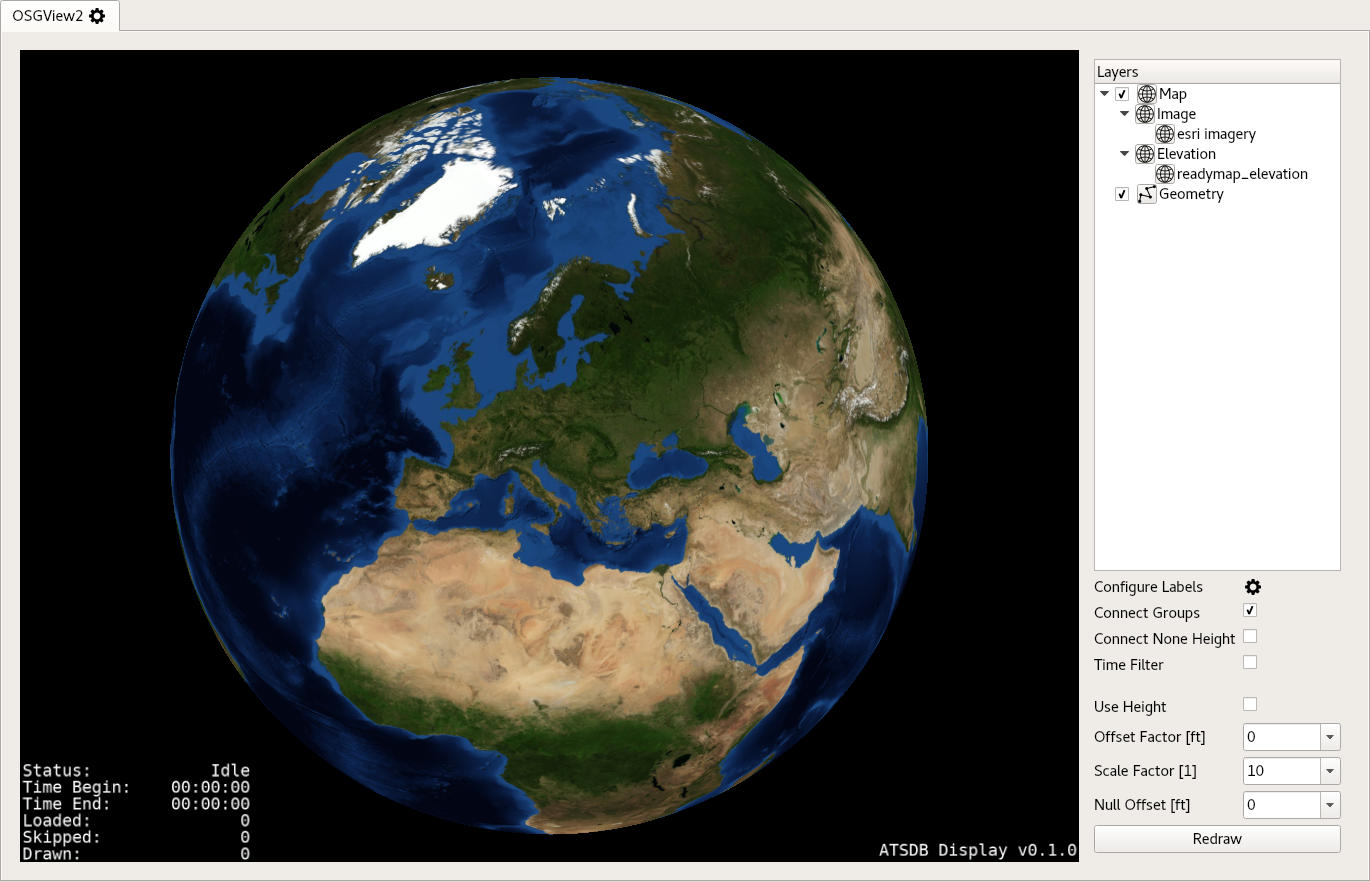
\includegraphics[width=18cm,frame]{../screenshots/osgview_arcgis.png}
  \caption{OSG View Arcgis map}
\end{figure}

\newpage
\paragraph{Minimal Map}

This minimal map shows national borders based on an ESRI shapefile, provided by Bjorn Sandvik on \url{thematicmapping.org}. In the AppImage application use 'minimal.earth', in newer ones the 'minimal\_new.earth' file should be used.

\begin{figure}[H]
    \hspace*{-2cm}
    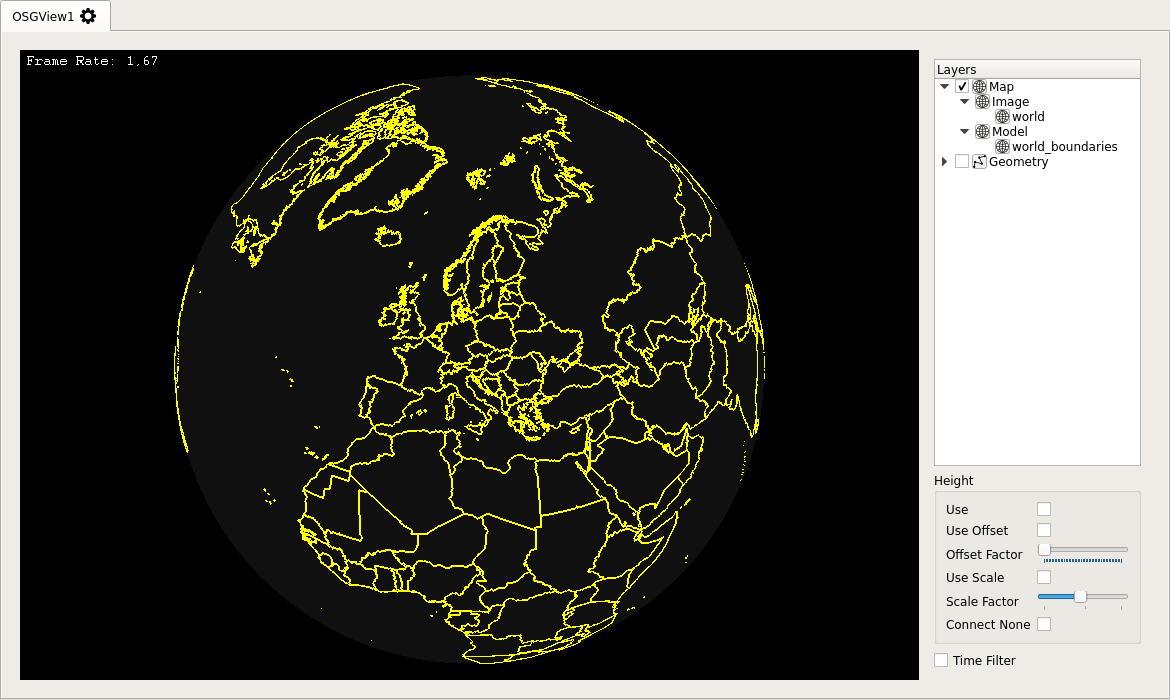
\includegraphics[width=18cm,frame]{../screenshots/osgview_minimal.png}
  \caption{OSG View minimal map}
\end{figure}

\newpage
\paragraph{Open Street Map}

This very useful map shows map data from \url{https://www.openstreetmap.org/}.

\begin{figure}[H]
    \hspace*{-2cm}
    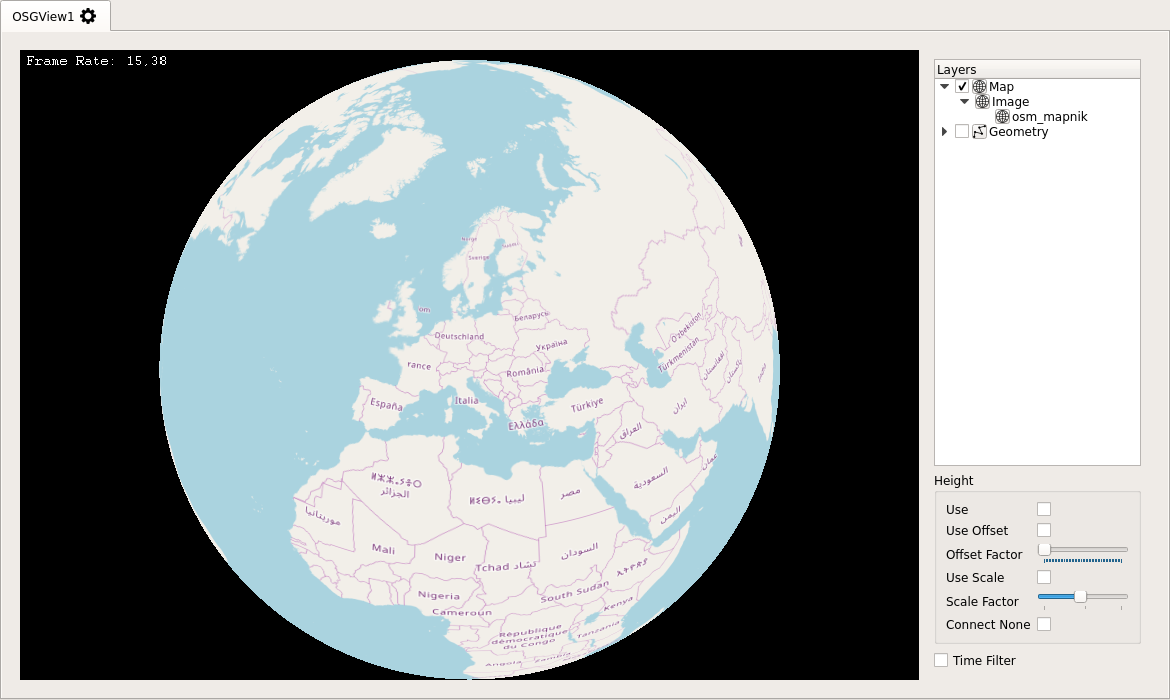
\includegraphics[width=18cm,frame]{../screenshots/osgview_osm.png}
  \caption{OSG View OpenStreetMap}
\end{figure}

It is possible to zoom in to a very high level of detail, to even inspect airport layouts.

\begin{figure}[H]
    \hspace*{-2cm}
    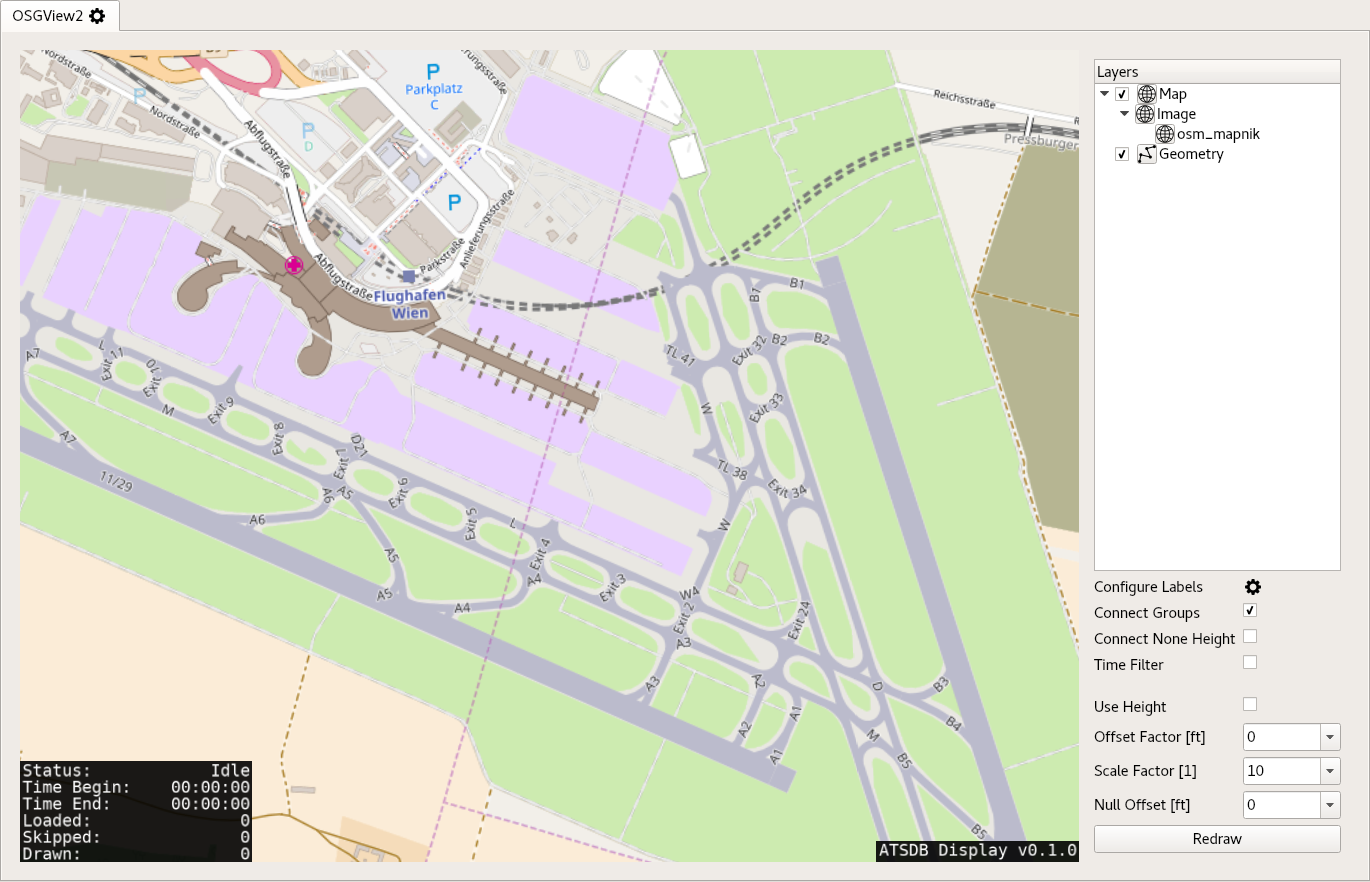
\includegraphics[width=18cm,frame]{../screenshots/osgview_osm_vienna.png}
  \caption{OSG View OpenStreetMap Vienna Airport}
\end{figure}

\newpage
\paragraph{ReadyMap}

This map also shows satellite data, from \url{http://web.pelicanmapping.com/readymap-tiles/}. It includes an elevation layer, so ground elevation is observable.

\begin{figure}[H]
    \hspace*{-2cm}
    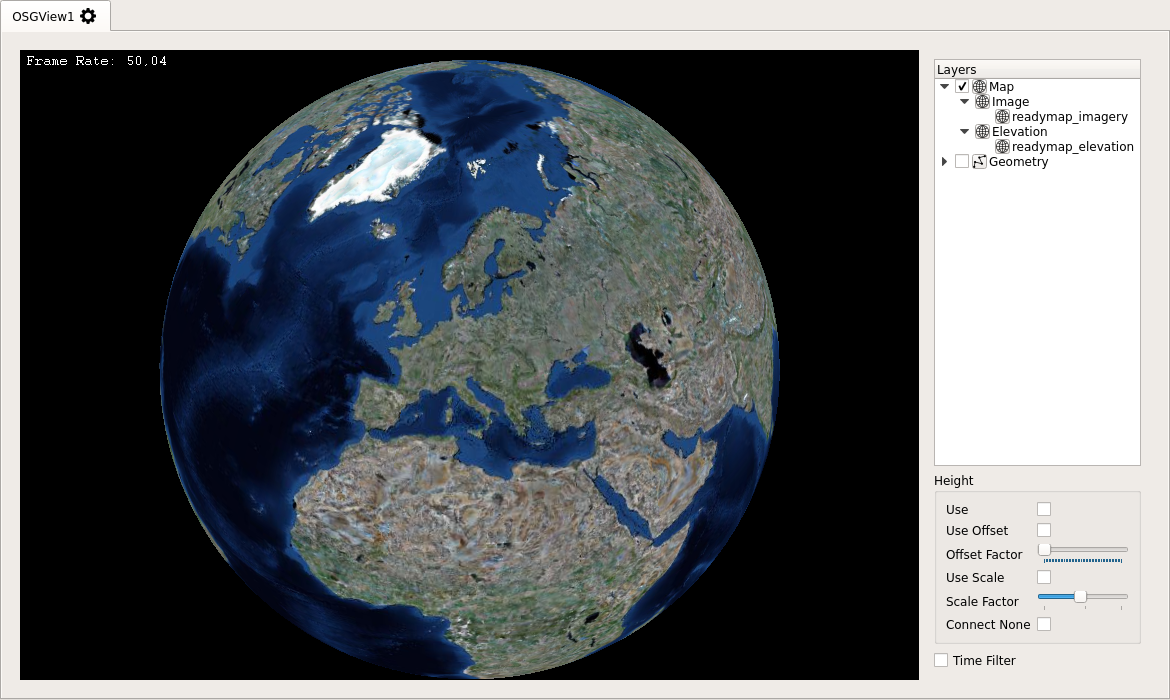
\includegraphics[width=18cm,frame]{../screenshots/osgview_ready.png}
  \caption{OSG View ReadyMap}
\end{figure}


\paragraph{ReadyMap Detailed}

This map shows the same data as ReadyMap, but to a higher detail level.

\begin{figure}[H]
    \hspace*{-2cm}
    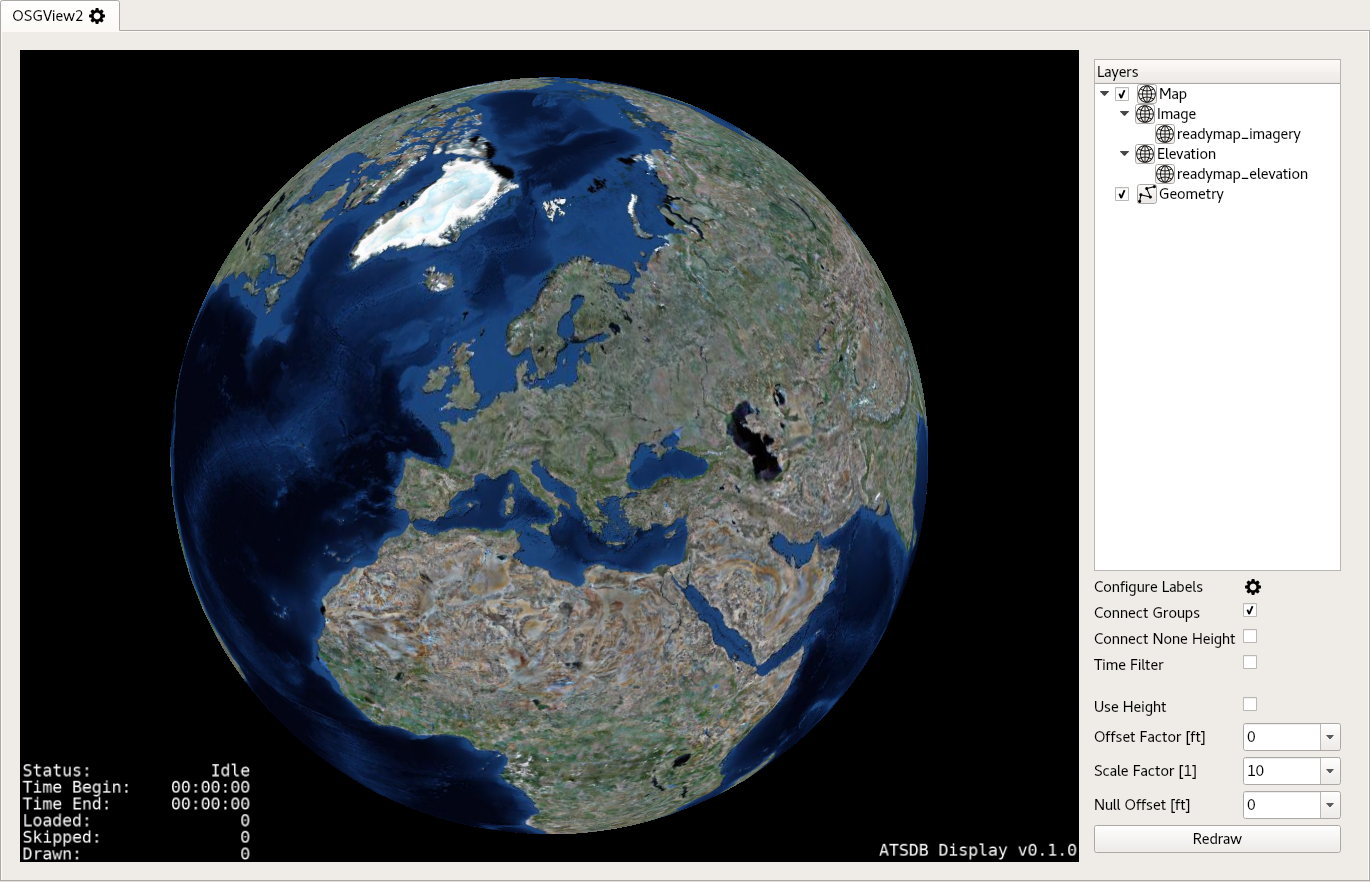
\includegraphics[width=18cm,frame]{../screenshots/osgview_ready_detail.png}
  \caption{OSG View ReadyMap detailed}
\end{figure}


\begin{figure}[H]
    \hspace*{-2cm}
    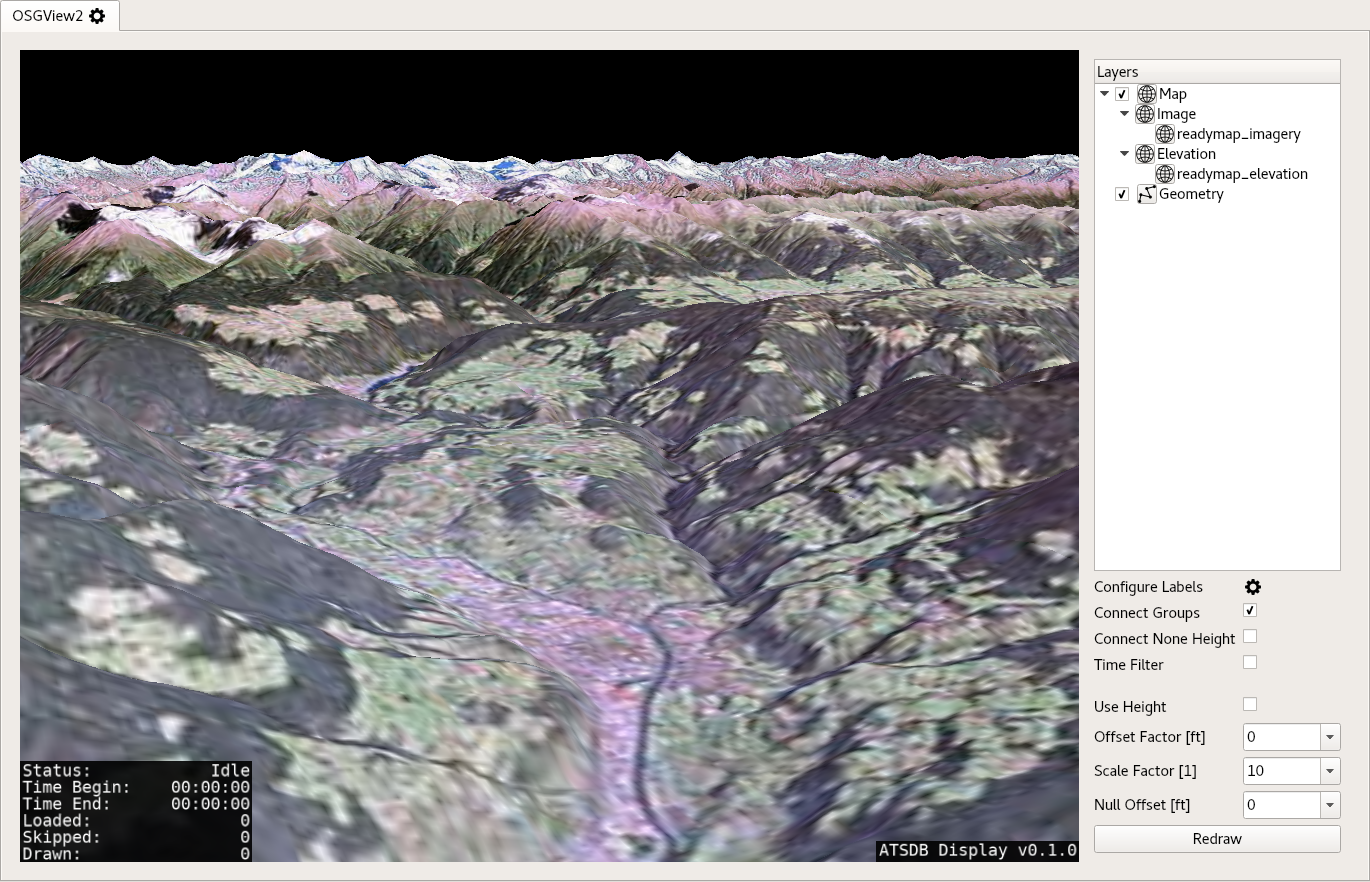
\includegraphics[width=18cm]{../screenshots/osgview_readymap_elav.png}
  \caption{OSG View ReadyMap detailed elevation}
\end{figure}


\subsubsection{Loading Data}
To load data, trigger a loading action from the Management widget. The data will be loaded as with the Listbox View, and displayed during the loading process. 

\begin{figure}[H]
    \hspace*{-2cm}
    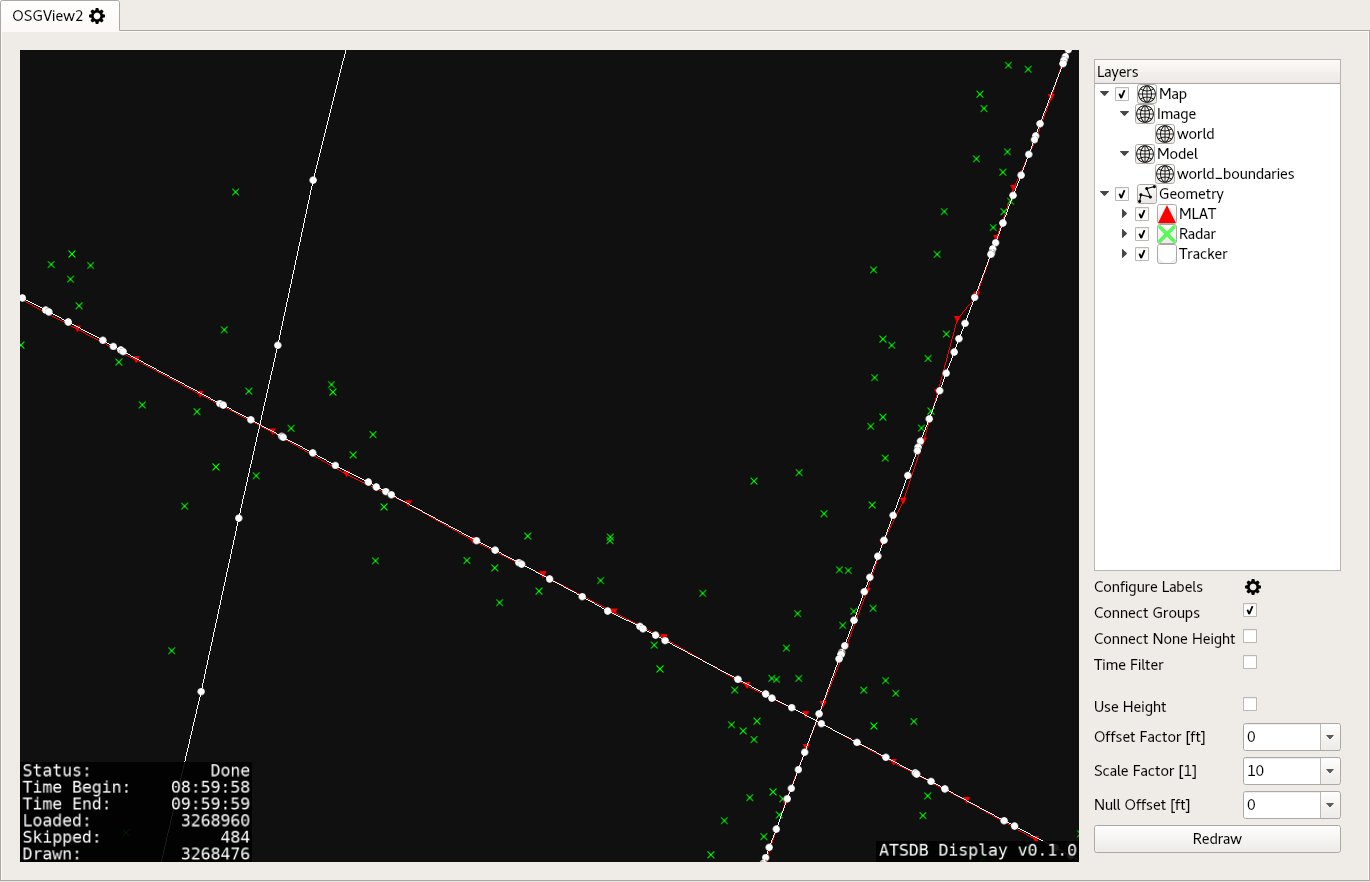
\includegraphics[width=18cm,frame]{../screenshots/osgview_data.png}
  \caption{OSG View data display}
  \label{fig:osgview_data}
\end{figure}

Please note that since currently only an example dataset is used, until real surveillance data can be made available.

Now, the loaded data is displayed in the following manner: For each DBO, a list of sensors exist, which supply the shown target reports. In the Geometry layers, the data is grouped as follows: Database Object $\rightarrow$ Sensor $\rightarrow$ Group. \\

For each DBO, a default display configuration is set:

\begin{itemize}
 \item ADS-B: Blue square
 \item MLAT: Red triangle
 \item Radar: Green cross
 \item Tracker: White circle
\end{itemize}

A sensor is of course a defined data source, e.g. a specific radar. A group currently is defined by a track number, and is connected by lines. If no track number is defined, the data is put into the 'Unassociated' group and not connected by lines.

\subsubsection{Layer Operations}

In the Layers widget, a number of operations are possible for each tree item.

\begin{table}[H]
  \center
  \begin{tabular}{ | l | l | l |}
    \hline
    \textbf{Operation} & \textbf{Trigger} &  \textbf{Description} \\ \hline
    View sub-items & Triangle & Opens or closes view of the sub-items \\ \hline
    Display item & Checkbox & Enables or disables display of items (and all sub-items) \\ \hline
    Display context menu & Click on symbol & Opens the items context menu \\ \hline
  \end{tabular}
  \caption{Layer operations}
\end{table}

The context menu allows several actions to be performed on an item. If an item has sub-items, the same action will automatically be performed on the child items.

\begin{figure}[H]
    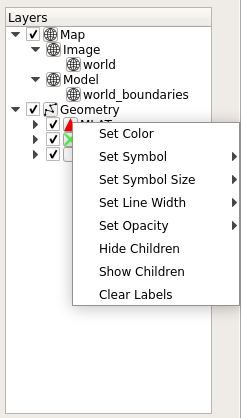
\includegraphics[width=5cm,frame]{../screenshots/osgview_layer_context_menu.png}
  \caption{OSG View layer context menu}
\end{figure}

\begin{itemize}
 \item Set Color: Open colour dialog to set the items colour
 \item Set Symbol: Set the items symbol to one of the following values:
\begin{itemize}
 \item Cross
 \item Circle
 \item Square
 \item Triangle
\end{itemize}
 \item Set Symbol Size: Set the symbols size
 \item Set Line Width: Set the line width
 \item Set Opacity: Set the items opacity
 \item Hide children: Disable display off all children
 \item Show Children: Enable display of all children
 \item Clear Labels: Removes all labels
\end{itemize}

Please note that only the main Map item has a context menu, and only allows setting of map files and changing the opacity.

\subsubsection{Map Widget Data Operations}
\label{sec:osgview_data_operations}

Several data-related operations can be also performed in the map widget.

\begin{table}[H]
  \center
  \begin{tabular}{ | l | l | l |}
    \hline
    \textbf{Mouse Action} & \textbf{Key Action} &  \textbf{Description} \\ \hline
    LMB click & CTRL & Toggle label display of a single target report \\ \hline
    RMB click & CTRL & Show data context menu \\ \hline
  \end{tabular}
  \caption{Map widget data operations}
\end{table}

\begin{figure}[H]
    \hspace*{-2cm}
    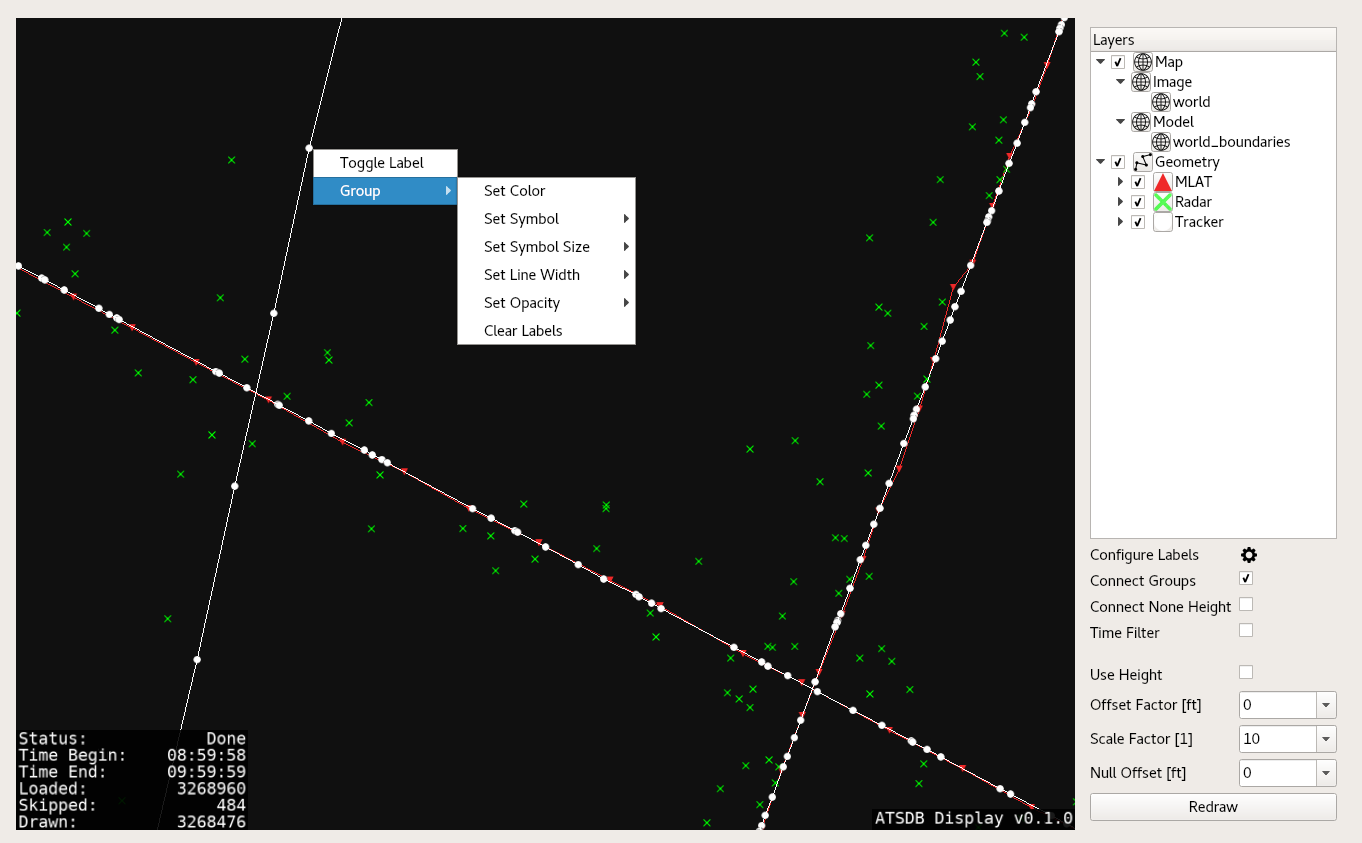
\includegraphics[width=18cm,frame]{../screenshots/osgview_data_operations.png}
  \caption{OSG View data operations}
\end{figure}

The data context menu allows the following operations:

\begin{itemize}
 \item Toogle Label: Toggle label display of a single target report
 \item Group: Same operations as on the item's group layer item
\end{itemize}

\subsubsection{Data Labeling}

Using the operations described in the previous section, labels can be shown for target reports.

\begin{figure}[H]
    \hspace*{-2cm}
    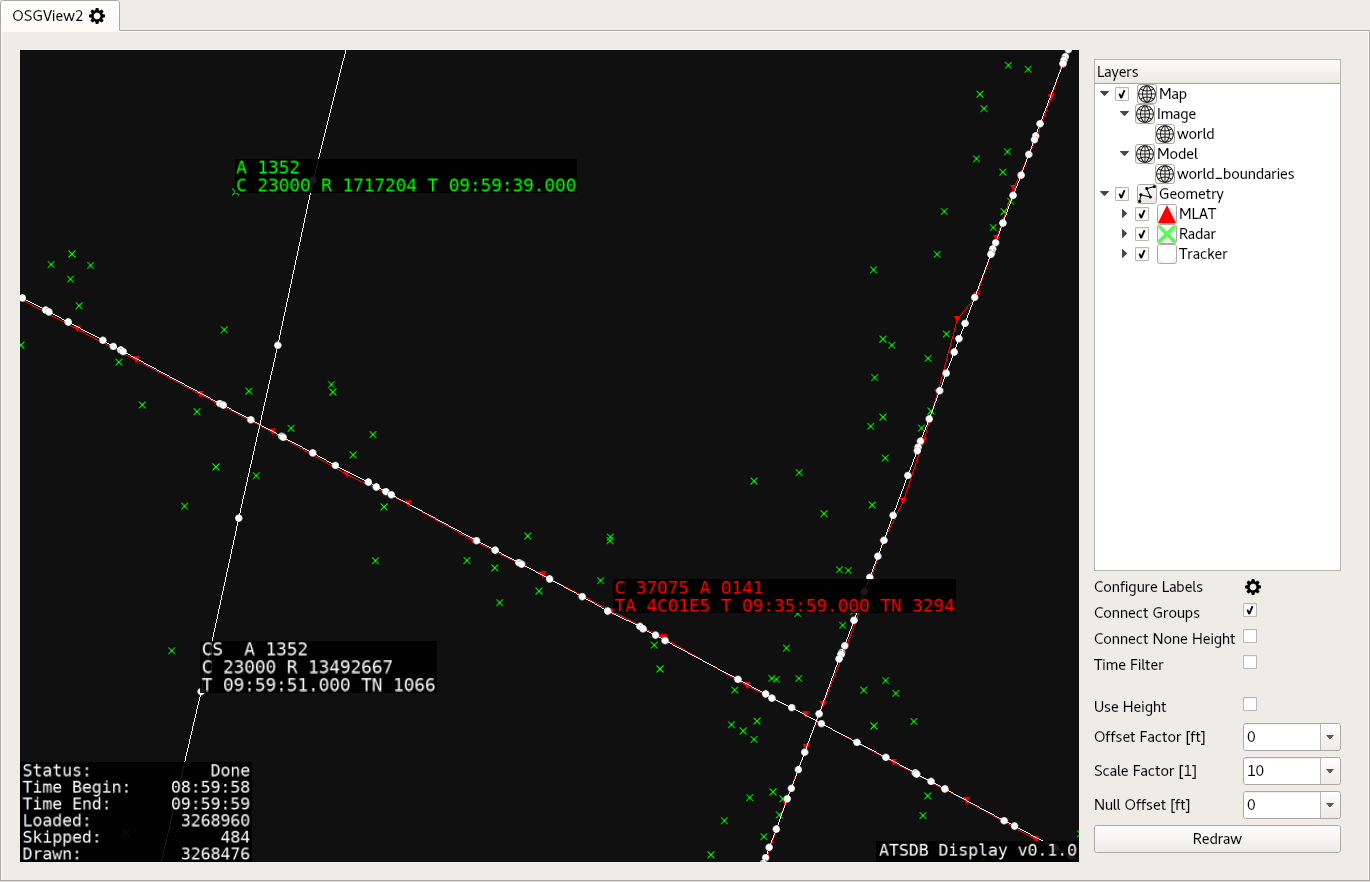
\includegraphics[width=18cm,frame]{../screenshots/osgview_labels.png}
  \caption{OSG View Labels}
\end{figure}

Using the ``Configure Labels'' button, the following operations are supported:

\begin{itemize}
 \item Clear: Clears all labels
 \item Edit: Edits which variables are shown, for each DBO
 \item Line Break: Sets after how many variable entries a line break is used
 \item Background color: Sets the background colour of the label
\end{itemize}

When a edit window for a DBO label definition is opened, a window like the following is shown:

\begin{figure}[H]
    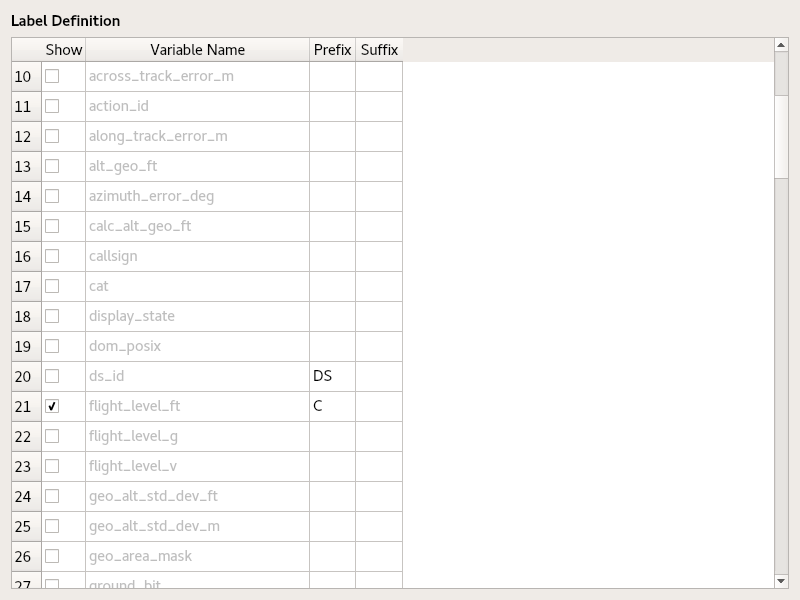
\includegraphics[width=12cm,frame]{../screenshots/osgview_label_edit.png}
  \caption{OSG View Label Editing}
\end{figure}

For each DBO, for each variable it can be selected if the value is presented (using the checkbox), and a prefix and suffix can be defined. The changes made to the prefix and suffix are made by double-clicking on the respective field, entering a new value, and setting the value by pressing enter. Upon each change, the existing labels in the OSG View are updated automatically. \\

A few notes about labels:

\begin{itemize}
 \item The label definition and presentation is persisted in the configuration
 \item The label colour is always the same as the target report's
 \item A variable value is only shown if it is present (not NULL)
 \item Labels are shown at the target reports position, matched to the lower-left corner
 \item A line break is given after the configured number of values. If values are not shown (NULL), the line break is still made at the same postion, to keep the value shown in the same line for all target reports.
\end{itemize}

\subsubsection{Time Filter}

Once activated using the ``Time Filter'' checkbox,  the time filter facilitates that only target reports within a specific time window are shown.


\begin{figure}[H]
    \hspace*{-2cm}
    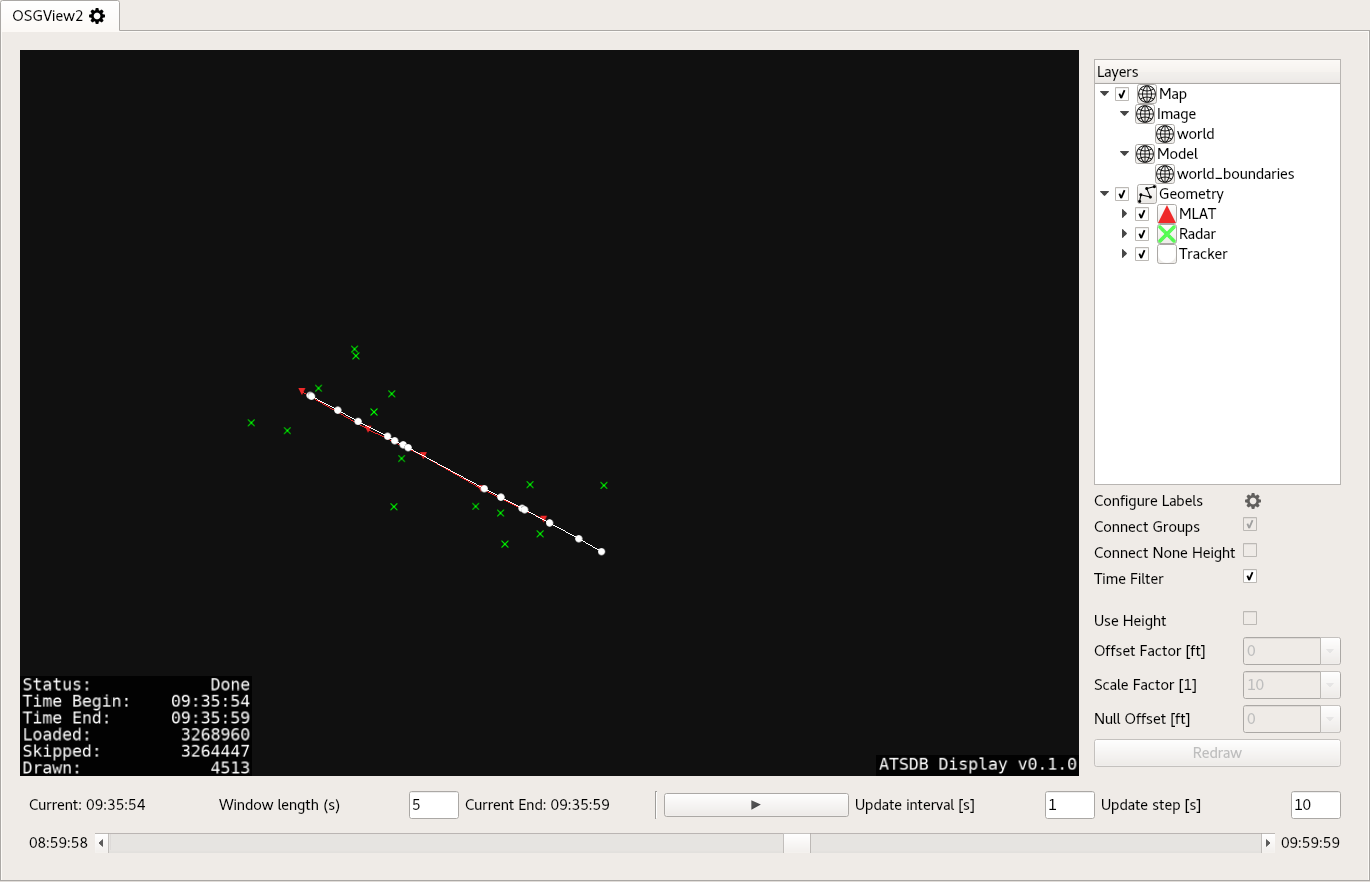
\includegraphics[width=18cm,frame]{../screenshots/osgview_time_filter.png}
  \caption{OSG View time filter}
  \label{fig:osgview_time_filter}
\end{figure}

The following items exist:

\begin{itemize}
 \item Current: The start of the time window
 \item Window length (s): Duration of the display time window
 \item Current End: The end of the time window
 \item Play button: Start/Stop the auto-play mode
 \item Update interval [s]: Auto-play mode update interval
 \item Update step [s]: Auto-play mode update step
 \item Scrollbar: Manual time-scrolling
\end{itemize}

During usage of the time filter, changes in the Configuration Widget was suppressed, but changes in the Layers Widgets are possible.

\subsubsection{Depth Check}

Once activated using the ``Use Depth Check'' checkbox, during drawing it is checked wether data is occluded in the depicted scene. E.g. if target reports are ``below ground'', they are not shown.

\begin{figure}[H]
    \hspace*{-2cm}
    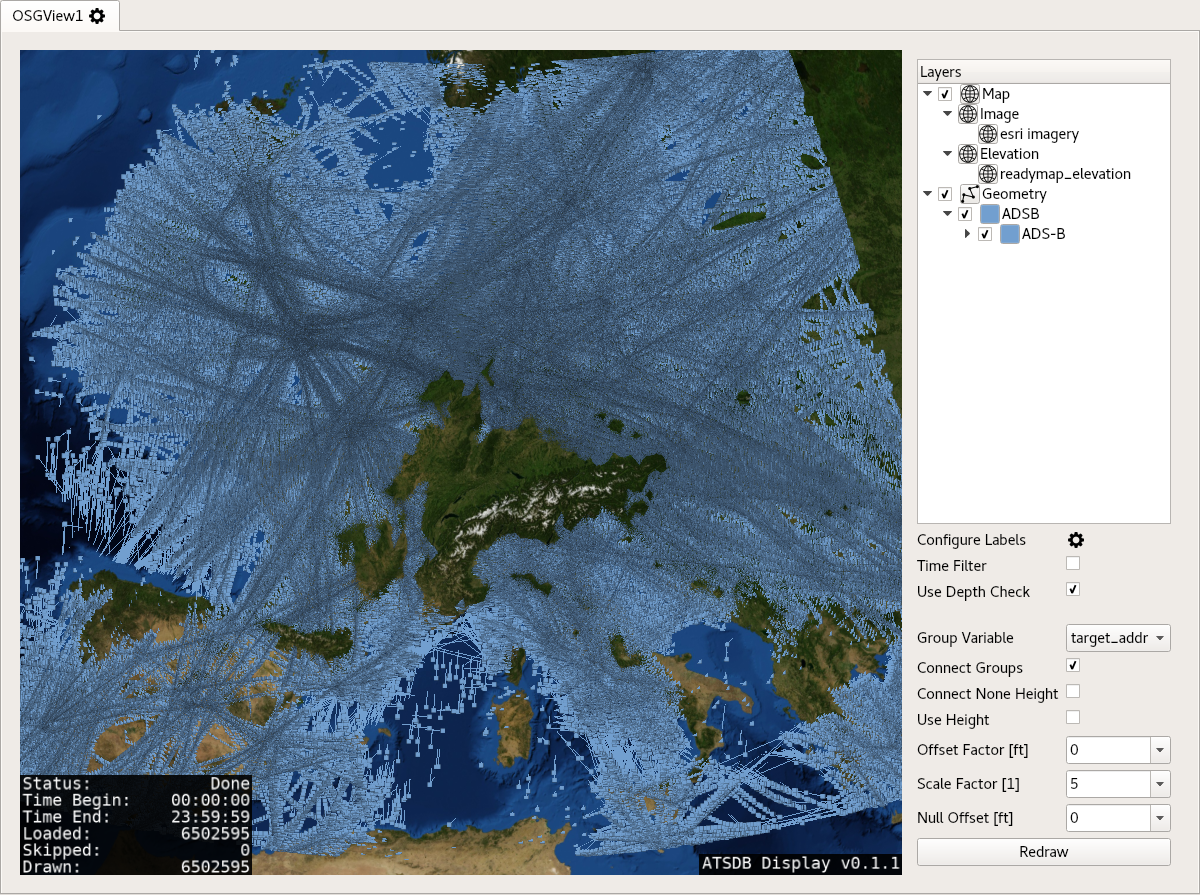
\includegraphics[width=18cm,frame]{../screenshots/osgview_depth_check.png}
  \caption{OSG View depth check}
\end{figure}

Please note that this should only be used in 3D, since in a 2D projection graphical artifacts exist. This is currently under investigation.

\subsubsection{Group Variable}

In this selectection the Meta DBOVariable used to create groups can be changed. Currently, only track number and Mode S address are supported. If e.g. data is shown, that has no track number but a Mode S address, this can be used to connect the respective targets.

\begin{figure}[H]
    \hspace*{-2cm}
    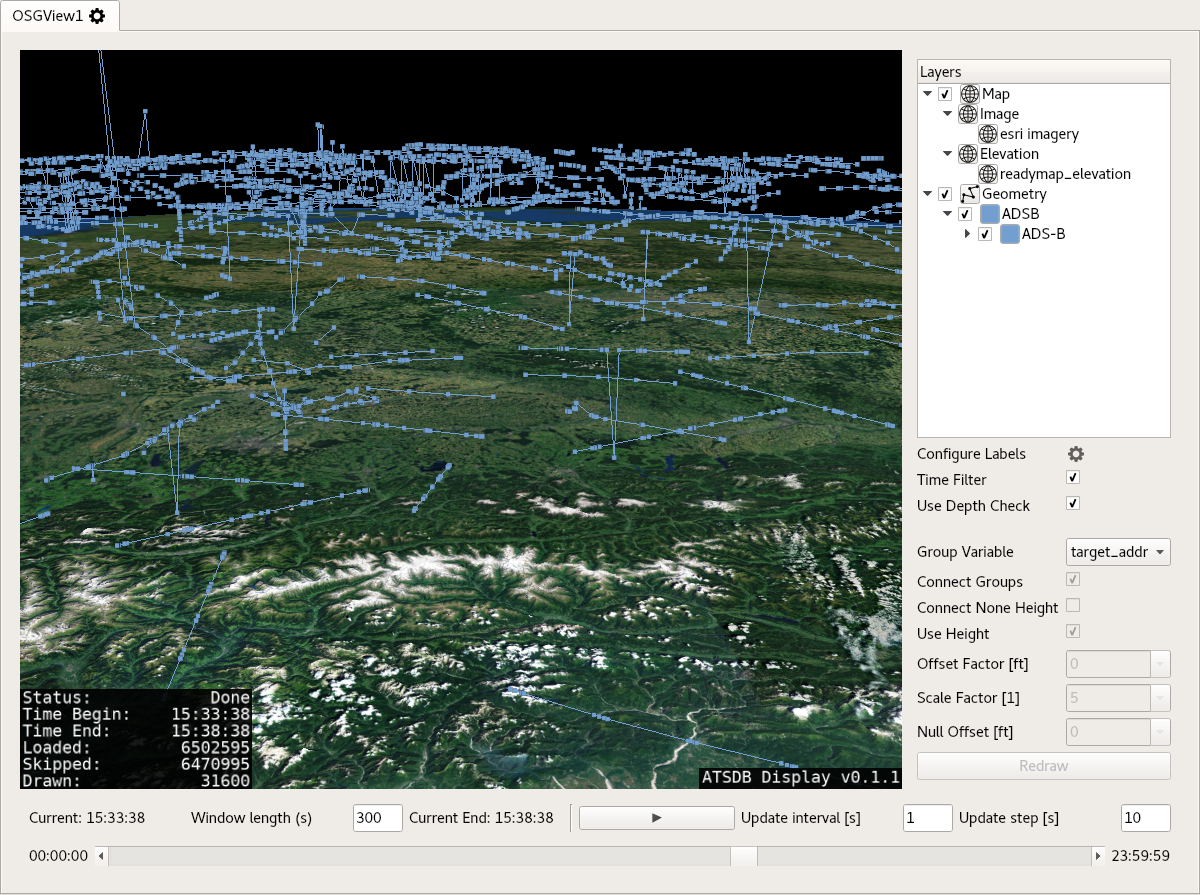
\includegraphics[width=18cm,frame]{../screenshots/osgview_group_variable.png}
  \caption{OSG View group variable}
\end{figure}


\subsubsection{Group Lines}

Grouping is currently performed on track number. If the ``Connect Groups'' checkbox is set, connection lines between all target reports in the same group are drawn, except for the ``Unassociated group'', where not track number was set.

\begin{figure}[H]
    \hspace*{-2cm}
    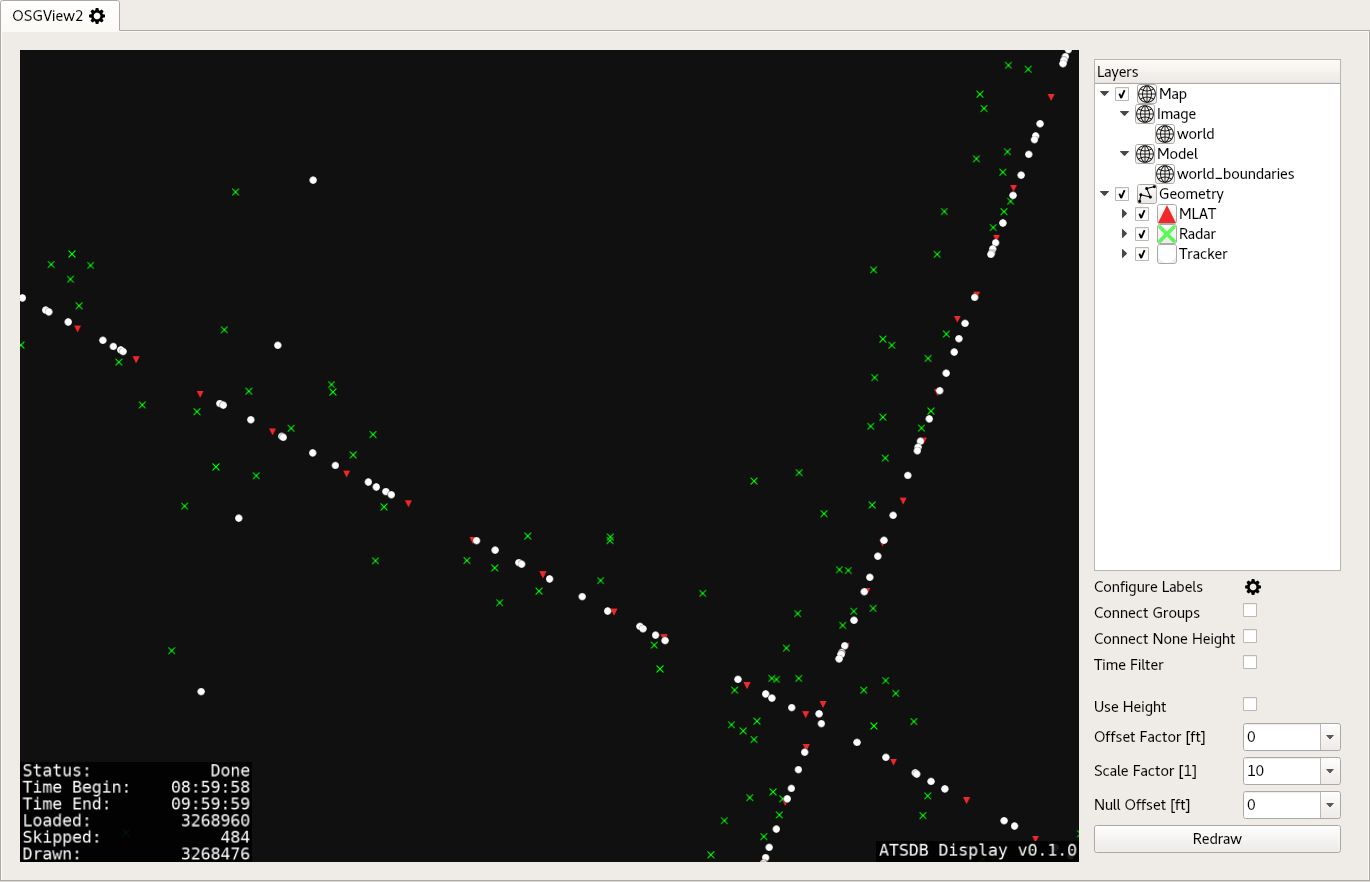
\includegraphics[width=18cm,frame]{../screenshots/osgview_no_lines.png}
  \caption{OSG View Data without lines}
\end{figure}

If the height information is used (3D view), if target reports without height information are connected, the lines clutter the display. The ``Connect None Height'' checkbox allows to set the behaviour. \\

Please \textbf{note} that changes both these values requires a manual redraw using the ``Redraw'' button.

\subsubsection{Height Operations}

Per default, a target reports height is not used for display, which is common in current air-traffic displays. However, in certain situation a true 3D display might be of interest to a user, and therefore several options where incorporated:

\begin{itemize}
 \item Use Height: Use the height based on Mode C $h_c$, transformed to meters
 \item Offset Factor: If height information is used, this factor $h_o$ is added to the height
 \item Scale Factor: If height information is used, this factor $h_s$ is used to multiply the height
 \item Null Offset: If height information is used, this factor $h_n$ is used for target reports without height information
\end{itemize}

Generally, if no height information is given (no Mode C code), the height is either $0$ or the height offset (if used). That means that those target reports appear to the on the ground. If connection lines are drawn between the ones in the air and those without, a lot of annoying lines are shown.

The formula to calculate the height (if existing) is as follows:

$$ h = h_o + h_s \cdot h_c [m]$$ 

If no height information is given:

$$ h = h_n [m]$$ 

Please note that upon changes to the height usage, a manual redraw has to be performed using the ``Redraw'' button.


\begin{figure}[H]
    \hspace*{-2cm}
    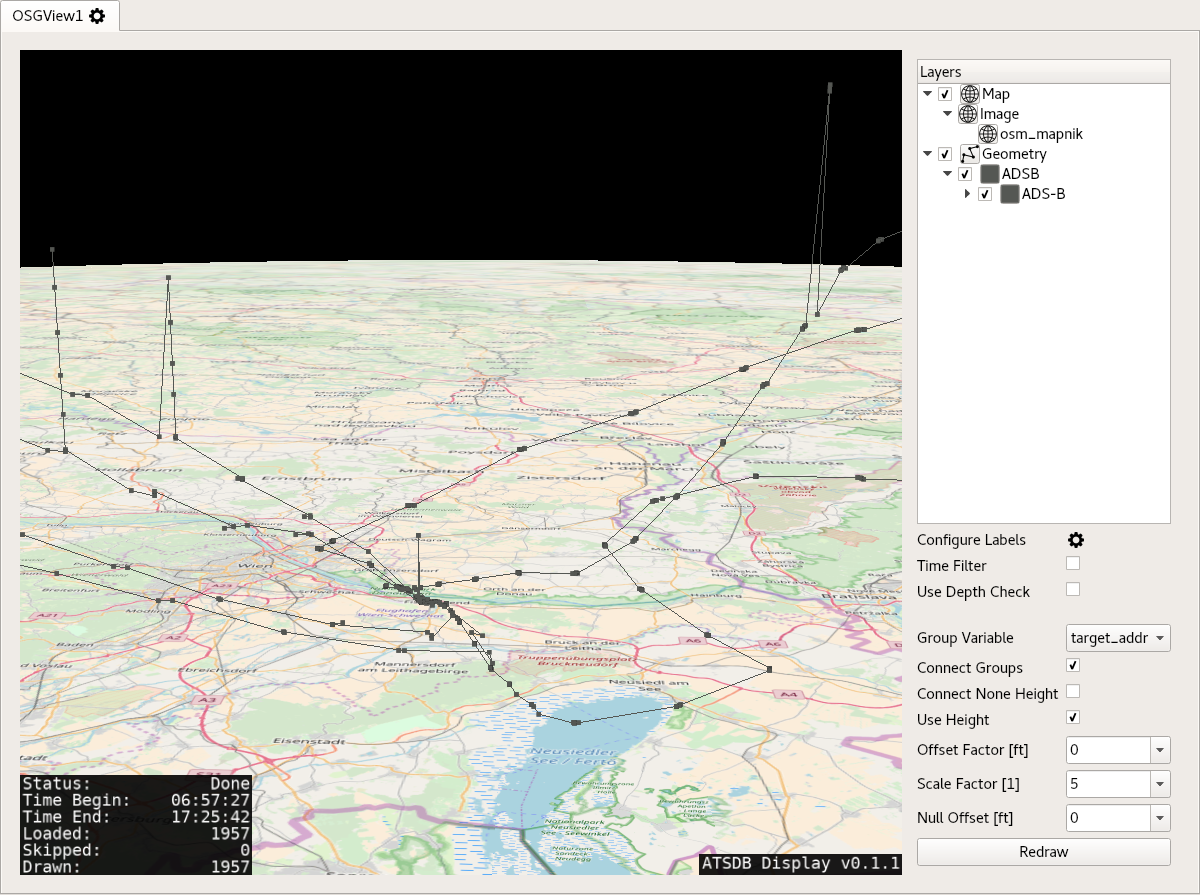
\includegraphics[width=18cm,frame]{../screenshots/osgview_use_height.png}
  \caption{OSG View use height}
\end{figure}

 
